\chapter{Solución propuesta}
\label{chap-solution}

En esta Sección se describen las técnicas aplicadas para lograr el seguimiento
de los jugadores. En primer lugar, se detallan algoritmos utilizados para
ignorar los elementos del fondo de la imagen en la Sección
\ref{sec:background-elimination}. Luego, se detalla cómo fue utilizado el
algoritmo contornos activos (ver \cite{fast-level-set}) y las modificaciones
que se le hicieron en la Sección \ref{sec:ac-extension}.

\section{Eliminación de fondo}

\label{sec:background-elimination}
Se evaluó que el análisis por contornos activos se beneficiaría de un análisis
previo que detecte e informe a la actualización del contorno sobre sectores de
los cuadros del video que sin duda no corresponden a las siluetas de los
objetos de interés para el seguimiento.

Con ese fin, se analizaron distintos métodos para extraer información adicional
de la imágen y detectar con el objetivo de ignorar sectores de la imágen que no
correspondan a jugadores con total certeza. A continuación se describen los
métodos evaluados.

\subsection{Tribuna y publicidades}
\label{subsec:crop-tribunas}

La técnica más simple de eliminación de sectores es una técnica de
\textit{recorte} que elimina de la imágen todo píxel ajeno a un polígono
(como puede ser un cuadrilátero) que bordea la cancha. En las Figuras
\ref{fig:crop-antes} y \ref{fig:crop-despues} se muestra el resultado
de aplicar esta técnica a uno de los videos utilizados en el trabajo.

\begin{figure}[H]
  \centering
    \begin{minipage}[t]{.45\textwidth}
      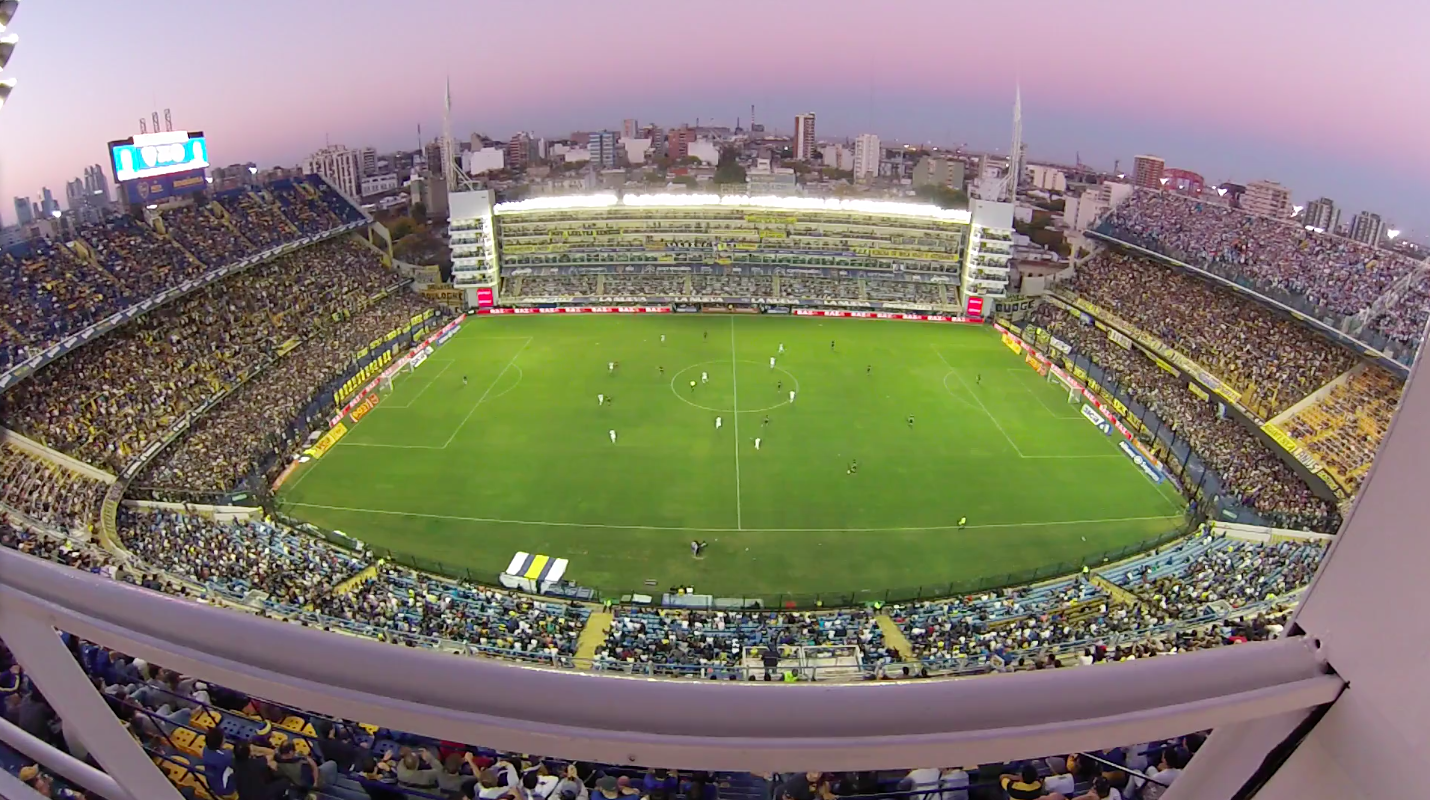
\includegraphics[width=\linewidth]{./images/Crop_Antes.png}
      \caption{Un cuadro del video de un partido entre Boca e Independiente.
      \label{fig:crop-antes}}
    \end{minipage}
    \begin{minipage}[t]{.45\textwidth}
      \centering
      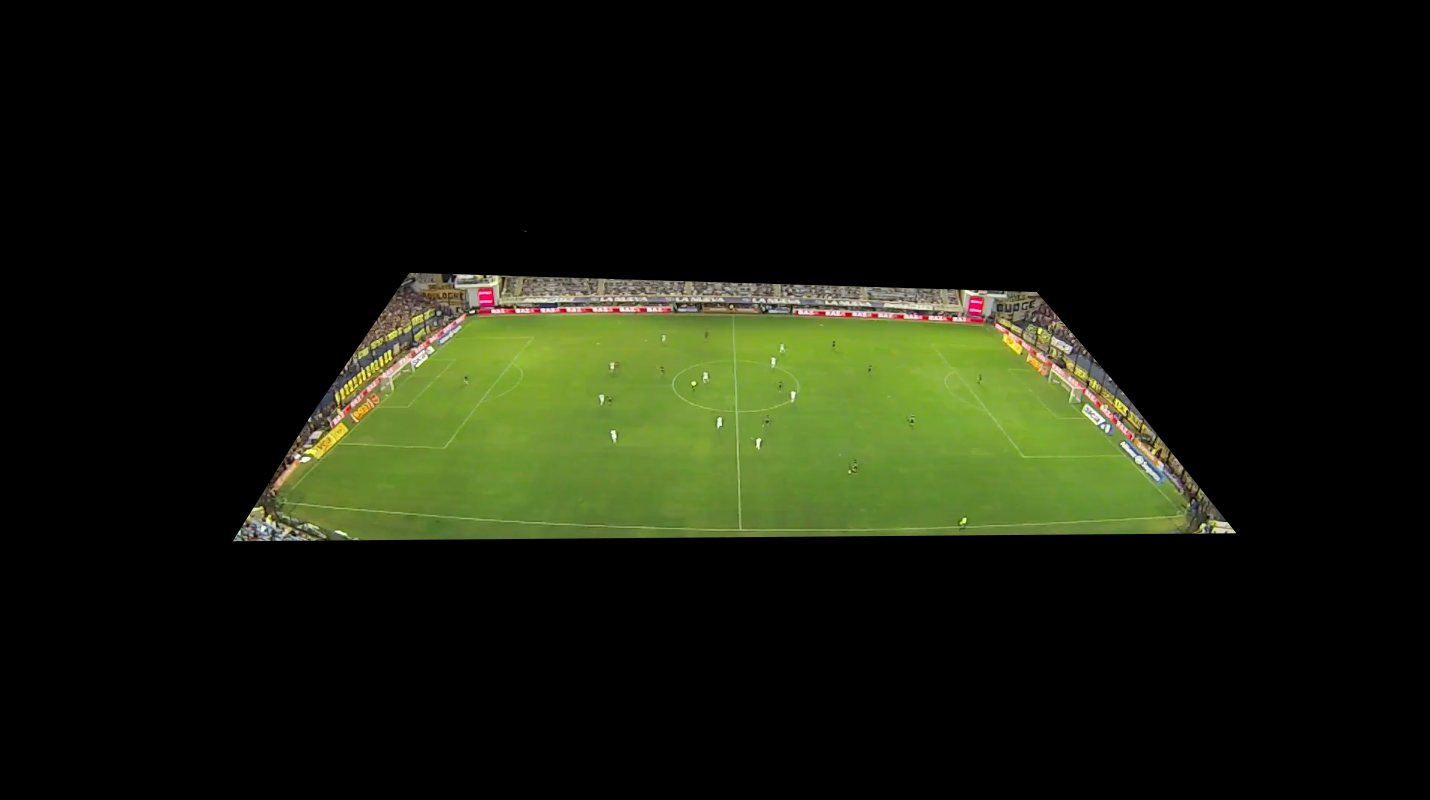
\includegraphics[width=\linewidth]{./images/Crop_Despues.png}
      \caption{El mismo cuadro, luego de aplicarle la operación \textit{recorte}.
      \label{fig:crop-despues}}
    \end{minipage}
\end{figure}

\subsection{Substracción de Fondo por Valor de Energía}

Se implementó el método de eliminación de fondo descripto en
\cite{papers-tanos}, para eliminación de sectores que corresponden al
verde del césped de la cancha o líneas pintadas sobre el mismo basado en una
medición de la variación del color de cada píxel (energía).

Este no resultó ser un método apropiado debido a que el sistema de codificación
del video generaba muchos falsos negativos, sobre todo \textit{glitches}
alrededor de las líneas de la cancha, lo que les otorgaba a estos puntos un
mayor valor de energía del que realmente tendrían. En la Figura \ref{fig:tanos-fondo-sin}
se muestra un recorte del primer cuadro del video de un partido entre Boca e Independiente.
En las figuras \ref{fig:tanos-fondo} y \ref{fig:tanos-fondo-broken} se muestra el
resultado de aplicar este algoritmo en ese mismo recorte. Se puede ver que en el cuadro
\#27 detecta muy bien el fondo, pero en el siguiente cuadro cambios en la imagen
hacen que descarte de manera erronea ciertas partes del fondo.

\begin{figure}[H]
  \centering
    \begin{minipage}[t]{.45\textwidth}
      
\includegraphics[width=\linewidth]{./images/tanos-fondo-f1.png}
      \caption{Recorte del cuadro \#1 del video de un partido entre Boca e Independiente
      \label{fig:tanos-fondo-sin}}
    \end{minipage}
    \begin{minipage}[t]{.45\textwidth}
      
\includegraphics[width=\linewidth]{./images/tanos-fondo-f27.png}
      \caption{Recorte del cuadro \#27 del video, con el fondo segun el algoritmo en azul.
      \label{fig:tanos-fondo}}
    \end{minipage}
    \begin{minipage}[t]{.45\textwidth}
      \centering
      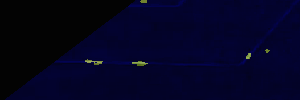
\includegraphics[width=\linewidth]{./images/tanos-fondo-f28.png}
      \caption{Recorte del cuadro \#28 del video, con el fondo segun el algoritmo en azul.
      \label{fig:tanos-fondo-broken}}
    \end{minipage}
\end{figure}

Otro problema encontrado con este algoritmo es que al basarse en cambios de color
puede considerar que un jugador que se encuentra estatico durante varios cuadros
es parte de fondo. Si bien los jugadores suelen estar en movimiendo durante el 
partido, esto no es tan cierto en el caso del arquero.

Por los motivos detallados, abandonamos el uso de este algoritmo en favor de las
tecnicas descriptas en la proximas secciones, \ref{sec:lineas} y \ref{sec:cesped}.

\subsection{Eliminación de Líneas}
\label{sec:lineas}

Se encontro que las lineas blancas que delimitan la cancha y sus distintas partes
presentan un problema para el seguimiento de los equipos con camisetas blancas o de
colores claros. Para evitar que el algoritmo de contornos activos considere que las
lineas son parte de un jugador, como en la figura \ref{fig:confusion-linea}.

% TODO: Tebex, esto no parece coincidir co nel codigo...
% TODO: esta bien que digas que probamos, pero no decis cual es el posta
% TODO: Decis "analisis morfologico" es muuuuy poco explicativo
Basado en la detección de líneas de Hough, se desarrolló un método similar que
detecta los tramos pintados de blanco en el césped de la cancha. El mismo
funciona aplicando un detector de bordes (se probaron resultados utilizando
tanto el método de Roberts como el de Canny), umbralizando el resultado, y
haciendo un análisis morfológico de las componentes conexas obtenidas luego de
la umbralización.

\begin{figure}[H]
  \centering
    \begin{minipage}[t]{.45\textwidth}
      
\includegraphics[width=\linewidth]{./images/confusion-linea.png}
      \caption{Resultado de aplicar el algoritmo sin eliminación de lineas
      \label{fig:confusion-linea}}
    \end{minipage}
\end{figure}

\subsection{Eliminación del césped}
\label{sec:cesped}

Para la eliminación del césped del campo de juego se requiere caracterizarlo
de alguna forma. Para esto, se realiza un analisis de los colores de
la imagen recortada, es decir la imagen resultante luego aplicar la técnica
de \textit{recorte}, detallada en \ref{subsec:crop-tribunas}, una vez seleccionados
los contornos iniciales de los jugadores. Sobre este cuadro, se calcula el valor
promedio y desvio estandard de todo pixel que no forme parte de los jugadores o
un elemento ya conocido del fondo (por ejemplo, las lineas). 

Con este valor, se considera parte del césped cualquier punto que no tenga las
caracteristicas de un jugador (segun definidas en la sección \ref{sec:caracteristicas}),
y se encuentre a menos de 3 desvios del color promedio calculado.

\section{Contornos activos}
\label{sec:ac-extension}

Como se explica en Sección \ref{sec:ac-problemas}, cuando los objetos de
interés son complejos, la utilización del color promedio como única
característica distintiva no alcanza. Es por esto que varias de las mejoras
planteadas al algoritmo de contornos activos giran en torno a la selección de
características para representar a los objetos de interés. Esta Sección
describe cambios que se han incorporado para hacer el algoritmo más efectivo
ante un video correspondiente a un partido de fútbol.

Si bien el color promedio resulta insuficiente para caracterizar correctamente
al objeto, puede utilizarse en complemento con otras características. Una opción
es la utilización de la varianza de color en el objeto de interés.

Además de estos indicadores estadísticos, se pueden utilizar varias valores
para caracterizar el objeto, en lugar de utilizar un solo valor como puede ser
el color promedio o la varianza. Para esto, por ejemplo, puede realizarse un
histograma de colores y seleccionar los picos más altos del histograma como
colores representativos del objeto.

\subsection{Características}
\label{sec:caracteristicas}

Se estudiaron varias posibilidades para la selección de características que
determinaran los contornos de los jugadores respecto al color de fondo.
Finalmente, se optó por utilizar tres características, correspondientes a los
valores de RGB de cada píxel. A continuación se detallan alternativas:
\begin{itemize}
  \item \textbf{Valores HSL}: Se tomaron, en vez de los valores de rojo, verde
    y azul, los valores de \textit{hue}, \textit{saturation} y
    \textit{lightning}.

  \item \textbf{Desviación Estándar}: Se tomaron seis características para cada
    píxel: color (RGB o HSL) y desviación estándar de ese píxel respecto a los
    demás píxeles en una ventana de 3x3 píxeles alrededor del mismo.

\end{itemize}

\subsubsection{Selección de características}

Las características de un jugador son seleccionadas en base a los valores
encontrados inicialmente dentro de un cuadrado de un ancho y alto especificado
por el operador, que depende del video siendo analizado. Entre los píxeles
abarcados por el área de ese cuadrado, se calcula el promedio y desvio estandard
de todos ellos. La caracteristica del jugador queda entonces definida por el
vector $v = (r_a, g_a, b_a, r_{dev}, g_{dev}, b_{dev})$, donde los primeros
tres valores representan el promedio de los componentes \textit{RGB} y los ultimos
tres el desvio standard de los componentes \textit{RGB}.

El vector de caracteristicas del fondo tiene la misma forma, y se construye
utilizando los valores calculados en la Sección \ref{sec:cesped}.

\subsubsection{Aprendizaje de valores}

Se realiza un aprendizaje simple para las características de cada contorno. En
cada cuadro, siendo las características de un contorno dado un vector
$\mathbf{v}$, se calcula el promedio de los valores de las características para
todos los píxeles pertenecientes al contorno y se lo denomina
$\hat{\mathbf{v}}$. A continuación se actualiza $\mathbf{v}$ y se lo reemplaza
por un nuevo valor $\mathbf{v_n}$ calculado de acuerdo a:

\[
  \mathbf{v_n} = \left(1-\alpha\right)\mathbf{v} + \alpha \hat{\mathbf{v}}
\]

Se toma un valor de $\alpha$ del orden de $10^{-2}$, es decir, se toma el $1\%$
de $\hat{\mathbf{v}}$. Esto evita la posibilidad de que se memorize cambios
no deseados, como lo podria ser una oclusion parcial, antes de su correción.

